% !TeX root = main.tex
\chapter{Introduction}
To survive in an ecosystem organisms need to adapt to the specific abiotic and biotic factors around them. This is particularly important for plants since they can not change their habitat during their lifespan. Adaptation can operate on different levels of the organisms from the adaptation of protein function to modifications in cell functions or whole tissue functions. But the underlying fundamental process that drives adaptation is the modification of the genetic material DNA.\\
Modifications on DNA level are called mutations and can be categorized in four different groups. A point mutation, which is the first group of mutations, is concerning just one single base pair. These changes the DNA sequence on one single point and therefore lead to changes of the transcribed mRNA. The second class of mutations are insertions. These insert a new sequence into the former DNA sequence and thus elongate it. These insertions can be of a variety of length from one single bp to a few hundred bp and even longer sequences can be added.  The contrasting class of mutations of insertions are deletions. Deletions lead to a reduction of base pairs in the former DNA strand. They can also vary in the length they delete. The last category of mutations are duplications. As implied by the name regions of the DNA get duplicated and inserted at a different position. The regions can be copied abnormally one or even more times.\\
These mutations are first of all just changes in the DNA but indirectly they impact all the resulting processes. The DNA first gets transcribed into mRNA. This process is not affected by the evolved mutations. But after the transcription the mRNA gets translated into proteins. In this step the impact of the mutations appear since a triplet codon gets translated into a specific amino acid. 
\begin{figure}[tb]
    \centering
    \begin{minipage}[h]{0.9\textwidth}
      \centering
      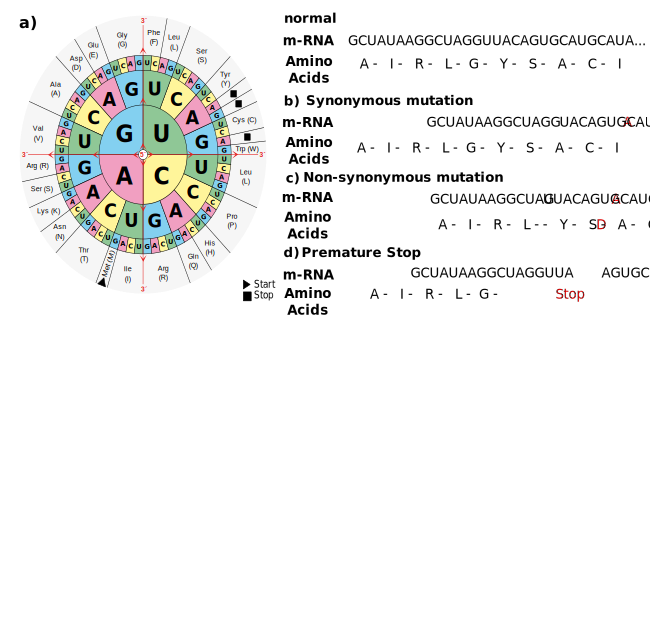
\includegraphics[width=0.9\textwidth]{images/Mutations.png}
      \caption{\textbf{Fundamental concepts of Translation of DNA into the Protein}\\
      a) The genetic code (image taken from \textcite{bresch2013})}
     \label{fig:Abb1.5}
    \end{minipage}
  \end{figure} 